\documentclass[../notes.tex]{subfiles}

\pagestyle{main}
\renewcommand{\chaptermark}[1]{\markboth{\chaptername\ \thechapter\ (#1)}{}}

\begin{document}




\chapter{Structure Determination}
\section{Intro + EA}
\begin{itemize}
    \item \marginnote{9/4:}Teaching team.
    \begin{itemize}
        \item Prof. Masha Elkin.
        \item Prof. Steve Buchwald.
        \item 8 Teaching Fellows (TFs).
    \end{itemize}
    \item Masha Elkin begins. Steve Buchwald and all TFs introduce themselves. Special roles:
    \begin{itemize}
        \item Head TF: Minh Le.
        \item Electronic TF (contact with questions on Canvas, Piazza, BACON): Angel Garcia-Ramirez.
    \end{itemize}
    \item In this class, you will learn\dots
    \begin{itemize}
        \item New things in organic chemistry;
        \item Old things at a deeper level;
        \item Real-world applications of chemistry.
    \end{itemize}
    \item Why study organic chemistry?
    \begin{itemize}
        \item Chemists manipulate matter, and that's awesome!
        \item By "manipulate matter," we mean making molecules, breaking molecules, making polymers, making detergents, and making sure that all of these things break down in the environment :)
    \end{itemize}
    \item Core questions.
    \begin{itemize}
        \item \emph{How} do we make molecules?
        \item What molecules \emph{should} we make?
    \end{itemize}
    \item Course logistics.
    \begin{itemize}
        \item Seven (7) units total (2 big units before the halfway mark \& 5 smaller units after).
        \item The units.
        \begin{itemize}
            \item Unit 1: How do we know what molecule(s) we have?
            \item Unit 2: How do electrons move?
            \item Units 3-7: How do we make molecules? How do reactions work?
        \end{itemize}
        \item Exams after units 1, 2, 4, and 6; final exam after unit 7.
        \item Questions? Ask your TF first, then the Head TF, then the profs (Masha \& Steve).
    \end{itemize}
    \item Prerequisites.
    \begin{itemize}
        \item Official prerequisites: 5.12 (equivalent to Orgo I, in case you took it elsewhere) \& Gen Chem.
        \item Recommended reading for review: Chapters 1-2 of the main textbook, referred to in these notes as \textcite{bib:Clayden}.
    \end{itemize}
    \item Grading.
    \begin{itemize}
        \item Your grade will (hopefully) be a reflection of your learning.
        \item There are no curves in this class or at MIT, so \emph{everyone can get an A!!!}
        \item How to improve your grade: Do problems!
        \begin{itemize}
            \item Problem sets (PSets) and recitation worksheets will be provided.
            \item You may also do as many textbook problems as you want. Feel free to buy the solutions manual, or borrow a copy from the ChemEd office\footnote{Located in 6-203.} to check your answers.
        \end{itemize}
    \end{itemize}
    \item How to learn organic chemistry.
    \begin{itemize}
        \item Analogy: Learning Orgo is like learning a language.
        \begin{itemize}
            \item Basic vocab and grammar that must be memorized. Examples: Drawing structures, curved arrow formalism, etc.
            \item Recognizing patterns and trends. Examples: Nucleophiles tend to have lone pairs (or be other regions of high electron density).
            \item Developing intuition.
            \item Practice, practice, practice! (Focus on drawing structures.)
        \end{itemize}
        \item Tips for success.
        \begin{itemize}
            \item Be active and participate in lecture, recitation, etc. Take notes while you're here!
            \item Practice \textbf{metacognition}, i.e., learn how you learn.
            \begin{itemize}
                \item Do you learn best in a crowded coffee shop, or in your own room? Would you rather recopy your notes, or read the textbook?
                \item Note that what works for somebody else may not work for you, and vice versa!
                \item Invest the time and effort that \emph{you} need to succeed. This may be more (or less) than other students, and that's ok!
            \end{itemize}
            \item Communicate with \emph{the whole} teaching team. They're here to help!!!
            \begin{itemize}
                \item Seek out accommodations as needed: It's the student's responsibility to ask.
            \end{itemize}
        \end{itemize}
    \end{itemize}
    \item \textbf{Metacognition}: Being aware of your own understanding.
    \item We now begin the content for Unit 1.
    \item Goal: Learn how to determine the chemical structure of a given organic compound.
    \item Why do we need to determine structures?
    \begin{figure}[h!]
        \centering
        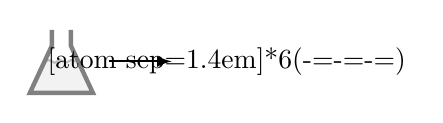
\begin{tikzpicture}
            \begin{scope}[xshift=-1cm,scale=0.4]
                \fill [gray!10] (-0.5,0) -- (-1,-1) -- (1,-1) -- (0.5,0);
                \draw [gray!50,thick,decorate,decoration={snake,segment length=4pt,amplitude=0.5pt}] (-0.5,0) -- (0.5,0);
    
                \draw [gray,ultra thick] (-0.3,1) -- (-0.3,0.5) -- (-1,-1) -- (1,-1) -- (0.3,0.5) -- (0.3,1);
            \end{scope}
            \draw [thick,-latex] (-0.4,0) -- (0.4,0);
            \node at (1.1,0) {\chemfig[atom sep=1.4em]{*6(-=-=-=)}};
        \end{tikzpicture}
        \caption{Why we study structure determination.}
        \label{fig:structureDeterminationRationale}
    \end{figure}
    \begin{itemize}
        \item With the naked eye, organic chemists see a flask with a colorless liquid. But we draw the skeletal diagram for benzene (which is a colorless liquid). What tools enable us to convert from the flask to the structure?
        \item Here's another reason: Suppose we run a brand new chemical reaction. Organic chemists do this all the time in research! How do we now what the product is? How do we know which atoms it contains, and in what arrangement?
    \end{itemize}
    \item Structure determination workflow.
    \begin{enumerate}
        \item Identify the atoms present.
        \begin{itemize}
            \item Questions to answer: What is the molecular formula?
            \item Relevant tools: Elemental analysis (EA) and mass spectrometry ("mass spec" or MS).
        \end{itemize}
        \item Identify the functional groups and substructures present.
        \begin{itemize}
            \item Questions to answer: Do we have ketones? Esters? Alcohols? Rings?
            \item Relevant tools: MS, infrared spectroscopy (IR), and nuclear magnetic resonance (NMR).\footnote{NMR is an organic chemist's best friend!}
        \end{itemize}
        \item Identify how all the functional groups fit together.
        \begin{itemize}
            \item Questions to answer: Are they close? Far apart? Ortho/meta/para? What stereochemistry?
            \item Relevant tools: NMR and X-ray diffraction.
        \end{itemize}
    \end{enumerate}
    \item We now begin talking about EA.
    \begin{itemize}
        \item History: Began development in the 1820s.
        \item Purpose: Determine which elements are present, and in what quantities (in a given sample).
    \end{itemize}
    \item In this course, we will apply EA to compounds containing carbon, hydrogen, and oxygen \emph{exclusively}.
    \begin{itemize}
        \item To reiterate, in an EA problem for this course, we will \emph{not} have to worry about any other elements.
        \item The typical EA technique for such compounds is \textbf{combustion analysis}.
    \end{itemize}
    \item \textbf{Combustion analysis}: Burn the sample and measure the products.
    \begin{itemize}
        \item All \ce{C} in the sample becomes \ce{CO2}.
        \item All \ce{H} in the sample becomes \ce{H2O}.
        \item \ce{O} is then determined via process of elimination, explained as follows.
    \end{itemize}
    \item Advanced techniques (beyond the scope of this class): Nitrogen to \ce{NO} or \ce{NO2}, sulfur to \ce{SO2}, etc.
    \item A schematic of combustion analysis.
    \begin{figure}[h!]
        \centering
        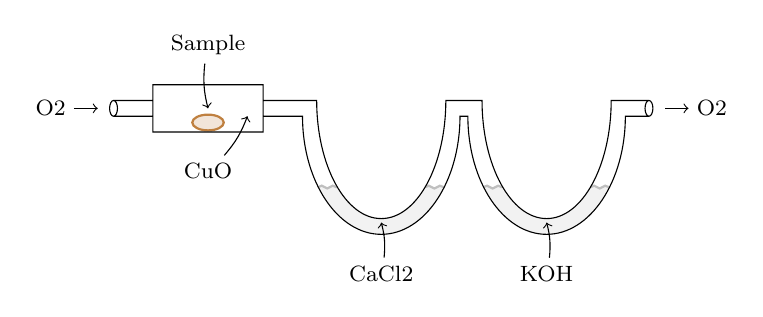
\begin{tikzpicture}
            \footnotesize
            \filldraw [draw=brown,thick,fill=brown!20] (0,-0.18) ellipse (2mm and 1mm);
            \node at (0,0.8) {Sample}
                edge[bend right=10,->] (0,0)
            ;
            \node at (0,-0.8) {\ce{CuO}}
                edge[bend right=10,->] (0.5,-0.1)
            ;
    
            \fill [gray!10] (1.4,-1)
                -- ({1.4+0.24},-1)
                arc[start angle=-140,end angle=-40,x radius=0.73cm,y radius=1.12cm]
                -- ({1.4+1.6},-1)
                arc[start angle=-40,end angle=-140,x radius=1.04cm,y radius=1.66cm]
                -- cycle
            ;
            \draw [gray!50,thick,decorate,decoration={snake,segment length=4pt,amplitude=0.5pt}] (1.4,-1) -- (1.64,-1);
            \draw [gray!50,thick,decorate,decoration={snake,segment length=4pt,amplitude=0.5pt}] (2.76,-1) -- (3,-1);
            \node at (2.2,-2.1) {\ce{CaCl2}}
                edge[bend right=10,->] (2.2,-1.45)
            ;
            \fill [gray!10] (3.5,-1)
                -- ({3.5+0.24},-1)
                arc[start angle=-140,end angle=-40,x radius=0.73cm,y radius=1.12cm]
                -- ({3.5+1.6},-1)
                arc[start angle=-40,end angle=-140,x radius=1.04cm,y radius=1.66cm]
                -- cycle
            ;
            \draw [gray!50,thick,decorate,decoration={snake,segment length=4pt,amplitude=0.5pt}] (3.5,-1) -- ({3.5+0.24},-1);
            \draw [gray!50,thick,decorate,decoration={snake,segment length=4pt,amplitude=0.5pt}] ({3.5+1.6-0.24},-1) -- ({3.5+1.6},-1);
            \node at (4.3,-2.1) {\ce{KOH}}
                edge[bend right=10,->] (4.3,-1.45)
            ;
    
            \draw
                (-1.2,0) ellipse (0.5mm and 1mm)
                (-1.2,0.1)  -- (-0.7,0.1)
                (-1.2,-0.1) -- (-0.7,-0.1)
                (-0.7,-0.3) rectangle (0.7,0.3)
                (0.7,-0.1) -- (1.2,-0.1)
                    arc[start angle=-180,end angle=0,x radius=1cm,y radius=1.5cm]
                    -- ++(0.1,0)
                    arc[start angle=-180,end angle=0,x radius=1cm,y radius=1.5cm]
                    -- ++(0.3,0)
                (0.7,0.1) -- (1.38,0.1)
                    arc[start angle=-180,end angle=0,x radius=0.82cm,y radius=1.5cm]
                    -- ++(0.46,0)
                    arc[start angle=-180,end angle=0,x radius=0.82cm,y radius=1.5cm]
                    -- ++(0.48,0)
                (5.6,0) ellipse (0.5mm and 1mm)
            ;
            \node at (-2,0) {\ce{O2}}
                edge [->] (-1.4,0)
            ;
            \node at (6.4,0) {\ce{O2}}
                edge [<-] (5.8,0)
            ;
        \end{tikzpicture}
        \caption{Combustion analysis schematic.}
        \label{fig:combustionAnalysis}
    \end{figure}
    \begin{itemize}
        \item Burn the sample in the presence of an oxidant such as cupric oxide (\ce{CuO}).
        \item Flow \ce{O2} into the combustion chamber to facilitate burning as well.
        \item The combusted gas then flows through a series of reaction containers.
        \begin{itemize}
            \item The first one contains a desiccant (like \ce{CaCl2}) that absorbs the water.
            \item The second one contains a base (like \ce{KOH}) that absorbs the \ce{CO2}.
        \end{itemize}
        \item The remaining oxygen flows out the end.
    \end{itemize}
    \item The \emph{analysis} part of combustion analysis.
    \begin{itemize}
        \item The amount of \ce{H} is equal to the change in mass of the \ce{CaCl2}.
        \begin{equation*}
            \Delta\text{mass}(\ce{CaCl2}) = \text{mass}(\ce{H2O})
            \to \text{ratio}(\ce{H})
        \end{equation*}
        \item The amount of \ce{C} is equal to the change in mass of the \ce{KOH}.
        \begin{equation*}
            \Delta\text{mass}(\ce{KOH}) = \text{mass}(\ce{CO2})
            \to \text{ratio}(\ce{C})
        \end{equation*}
        \item The amount of \ce{O} is equal to the change in mass of the sample.
        \begin{equation*}
            \text{mass}(\text{sample})-\text{mass}(\ce{H})-\text{mass}(\ce{C}) = \text{mass}(\ce{O})
             \to \text{ratio}(\ce{O})
        \end{equation*}
        \item Result: We get an \textbf{empirical formula} of the form \ce{C_{$x$}H_{$y$}O_{$z$}}. Remember that this is \emph{not} (necessarily) the \textbf{molecular formula}; it is \emph{only} a ratio of elements.
    \end{itemize}
    \item EA example: Let's burn \SI{0.5}{\gram} of propanol (\ce{C3H8O}).
    \begin{itemize}
        \item Suppose we obtain \SI{0.600}{\gram} \ce{H2O} and \SI{1.09}{\gram} \ce{CO2}.
        \item This means that there was \SI{0.067}{\gram} (\ce{H}) and \SI{0.300}{\gram} (\ce{C}) in the sample. The remaining \SI{0.133}{\gram} must then be due to \ce{O}.
        \item Therefore, the elements exist in a 3:8:1 (C:H:O) ratio.
        \item Bonus: Convert the masses to a ratio via stoichiometry.
        \begin{itemize}
            \item $
                \SI{0.600}{\gram}\ \ce{H2O}
                \times\dfrac{\SI{1}{\mole}\ \ce{H2O}}{\SI{18.02}{\gram}\ \ce{H2O}}
                \times\dfrac{\SI{2}{\mole}\ \ce{H}}{\SI{1}{\mole}\ \ce{H2O}}
                \times\dfrac{\SI{1.01}{\gram}\ \ce{H}}{\SI{1}{\mole}\ \ce{H}}
                = \SI{0.067}{\gram}\ (\ce{H})
            $
            \item $
                \SI{1.09}{\gram}\ \ce{CO2}
                \times\dfrac{\SI{1}{\mole}\ \ce{CO2}}{\SI{44.01}{\gram}\ \ce{CO2}}
                \times\dfrac{\SI{1}{\mole}\ \ce{C}}{\SI{1}{\mole}\ \ce{CO2}}
                \times\dfrac{\SI{12.01}{\gram}\ \ce{C}}{\SI{1}{\mole}\ \ce{C}}
                = \SI{0.300}{\gram}\ (\ce{C})
            $
            \item $
                \SI{0.5}{\gram}\ \text{propanol}
                -\SI{0.067}{\gram}\ (\ce{H})
                -\SI{0.300}{\gram}\ (\ce{C})
                = \SI{0.133}{\gram}\ (\ce{O})
            $
        \end{itemize}
    \end{itemize}
    \item A note on the previous example.
    \begin{table}[h!]
        \centering
        \small
        \renewcommand{\arraystretch}{1.4}
        \begin{tabular}{l|cc|ccc}
            \textbf{Name} & Propanol & Methyl ethyl ether & Formaldehyde & Acetic acid & Glucose\\
            \textbf{Structure} &
                \footnotesize\chemfig[atom sep=1em]{-[:30]-[:-30]-[:30]OH} &
                \footnotesize\chemfig[atom sep=1em]{-[:30]-[:-30]O-[:30]} &
                \footnotesize\chemfig[atom sep=1em,baseline=0.8em]{H-[:30](=[2]O)-[:-30]H} &
                \footnotesize\chemfig[atom sep=1em,baseline=0.8em]{-[:30](=[2]O)-[:-30]OH} &
                \footnotesize\chemfig[atom sep=1em]{?(-[:190]HO)-[:-50,1.4](-[:170]HO)-[:10,1.5](-[:-55]OH)-[:-10,1.5](-[:10]OH)-[:130]O-[:190]?(-[:150,0.7]-[2]OH)}\\
            \textbf{Emp. formula} & \ce{C3H8O} & \ce{C3H8O} & \ce{CH2O} & \ce{CH2O} & \ce{CH2O}\\
            \textbf{Mol. formula} & \ce{C3H8O} & \ce{C3H8O} & \ce{CH2O} & \ce{C2H4O2} & \ce{C6H12O6}\\
        \end{tabular}
        \caption{Questions that EA can't answer.}
        \label{tab:EAmols}
    \end{table}
    \begin{itemize}
        \item EA has given us the empirical formula, but it has \emph{not} confirmed that the sample is propanol. For example, methyl ethyl ether has the same empirical formula!
        \item Additionally, we don't yet have the molecular formula. Consider, for instance, the breadth of compounds with empirical formula \ce{CH2O}!
        \item Takeaway: EA gives you the empirical formula; we need MS to get the molecular formula (we'll see this on Friday), and we may need even more to get the atomic connectivity.
    \end{itemize}
    \item Application of EA to real-world chemistry.
    \begin{itemize}
        \item A home furnace burns natural gas --- which is mostly methane (\ce{CH4}) --- for heat.
        \item \textbf{Ideal combustion}\footnote{You can learn more about in a chemical engineering/ChemE course.} corresponds to the reaction
        \begin{equation*}
            \ce{CH4 + O2 -> CO2 + H2O}
        \end{equation*}
        \item Real-world combustion is incomplete; you make
        \begin{equation*}
            \ce{CH4 + air -> CO2 + H2O + NO2 + CO}
        \end{equation*}
        \item When a technician comes to your home, they analyze the flue gas (i.e., your furnace exhaust).
        \begin{itemize}
            \item Their analysis could determine that our combustion has too much \ce{O2}, which is called "air rich." This is inefficient and doesn't yield enough heat.
            \item They could also determine that you have too much \ce{CO2} and \ce{CO}, which is called "fuel rich." This yields too much soot and \ce{CO}. \ce{CO} can be dangerous and lead to carbon monoxide poisoning, which makes you sleepy before it kills you.
        \end{itemize}
        \item To measure this flue gas, though, they have a little handheld elemental analysis device!
    \end{itemize}
    \item Note that there is a relation between ideal/real-world combustion and the \ce{CuO} oxidant in Figure \ref{fig:combustionAnalysis}: The \ce{CuO} ensures that when we combust our EA sample, all the carbon is fully oxidized to \ce{CO2}! Without it, some \ce{CO} would be formed, and our stoichiometry would be thrown off.
\end{itemize}




\end{document}